\documentclass[a4paper]{article}

\usepackage{marvosym}
\usepackage{url,parskip}			%formatting
\usepackage{tikz}
\usepackage{tkz-graph}

%better formatting of the A4 page
\usepackage{fullpage}
%An alternative to Layaureo can be usepackage{fullpage}
 
\usepackage{supertabular} 		%for Grades
\usepackage{titlesec}			%custom section

\usepackage{enumitem}
 
%Setup hyperref package, and colours for links
\usepackage{hyperref}

\begin{document}

\title{Graph Theory Assignment 1}
\author {
    Davies, Michael\\
    \and
    Goosen, Chris\\
    \and
    Laten, Matthew\\
    \and
    Sharwood, Bee\\
    \and
}
\maketitle

\subsection*{1.2 d)}
Firstly, we notice that to get from $Q_{t-1}$ to $Q_t$, we take the cartesian
product of $Q_{t-1}$ with $K_2$. This results in the number of vertices in
$Q_{t-1}$ being doubled. Since $Q_1 = K_1$ and the order of $Q_1$ is 2, we have
that the order of $Q_t$ is given by $2 \times 2 \times ... \times 2$ $t$ times,
or rather $ord(Q_t) = 2^t$.

To compute the size of $Q_t$, we interpret each vertex as a t-digit binary
string, which is adjacent to every binary string which differs from it by
exactly one place. Further, we notice that each vertex has degree $t$. Thus,
the sum of the degrees of $Q_t$ is given by
\begin{equation}
    \sum_{v \in V(Q_t)} deg(v) = t\cdot2^t
\end{equation}
Thus, the size is $\frac{t\cdot2^t}{2} = t\cdot2^t$.

\subsection*{1.4}

\subsection*{1.5}

\subsection*{1.6}

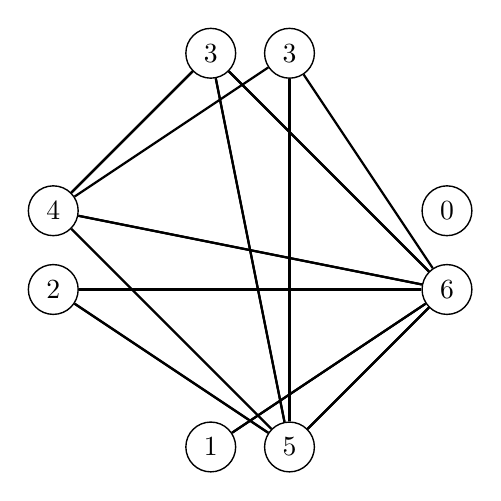
\begin{tikzpicture}
    \SetGraphUnit{2}
    \GraphInit[vstyle=Normal]
    \Vertex[x=0,y=2]{2}
    \Vertex[x=0,y=3]{4}
    \Vertex[x=2,y=0]{1}
    \Vertex[x=3,y=0]{5}
    \Vertex[x=5,y=2]{6}
    \Vertex[x=5,y=3]{0}
    \Vertex[x=2,y=5,L=3]{3A}
    \Vertex[x=3,y=5,L=3]{3B}
    \Edges(6, 1, 6, 2, 6, 4, 6, 5, 6, 3A, 6, 3B)
    \Edges(5, 2, 5, 3A, 5, 3B, 5, 4)
    \Edges(4, 3A, 4, 3B)
\end{tikzpicture}

\subsection*{1.7}

\subsection*{1.8}

\subsection*{1.9 c)}

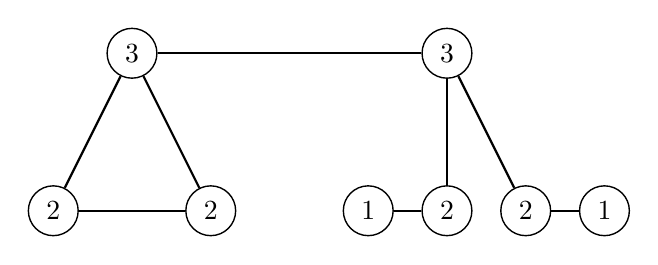
\begin{tikzpicture}
    \SetGraphUnit{2}
    \GraphInit[vstyle=Normal]
    \Vertex[x=0,y=0,L=2]{A}
    \Vertex[x=2,y=0,L=2]{B}
    \Vertex[x=1,y=2,L=3]{C}
    \Vertex[x=4,y=0,L=1]{D}
    \Vertex[x=5,y=0,L=2]{E}
    \Vertex[x=6,y=0,L=2]{F}
    \Vertex[x=7,y=0,L=1]{G}
    \Vertex[x=5,y=2,L=3]{H}
    \Edges(A, B, C, A)
    \Edges(C, H, E, D)
    \Edges(H, F, G)    
\end{tikzpicture}

\subsection*{1.9 d)}

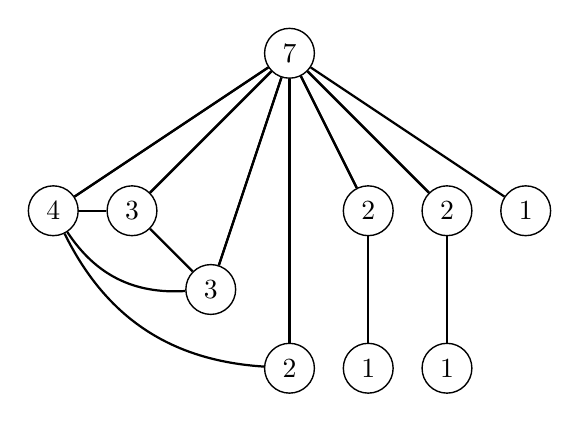
\begin{tikzpicture}
    \SetGraphUnit{2}
    \GraphInit[vstyle=Normal]
    \Vertex[x=3,y=4]{7}
    \Vertex[x=0,y=2]{4}
    \Vertex[x=1,y=2,L=3]{A}
    \Vertex[x=2,y=1,L=3]{B}
    \Vertex[x=3,y=0,L=2]{C}
    \Vertex[x=4,y=2,L=2]{D}
    \Vertex[x=5,y=2,L=2]{E}
    \Vertex[x=6,y=2,L=1]{F}
    \Vertex[x=4,y=0,L=1]{G}
    \Vertex[x=5,y=0,L=1]{H}
    \Edges(7, 4, 7, A, 7, B, 7, C, 7, D, 7, E, 7, F)
    \Edge[](4)(A)
    \Edge[style={bend right}](4)(B)
    \Edge[style={bend right}](4)(C)
    \Edge[](A)(B)
    \Edge[](D)(G)
    \Edge[](E)(H)    
\end{tikzpicture}

\subsection*{1.12} 

\subsection*{1.13}

\subsection*{1.15}

\subsubsection*{a)}

In the following images, $K_5$ is depicted with blue edges and $K_2$ is depicted with red edges. This is to improve the clarity of the images and make them more understandable. \\

$G + H$

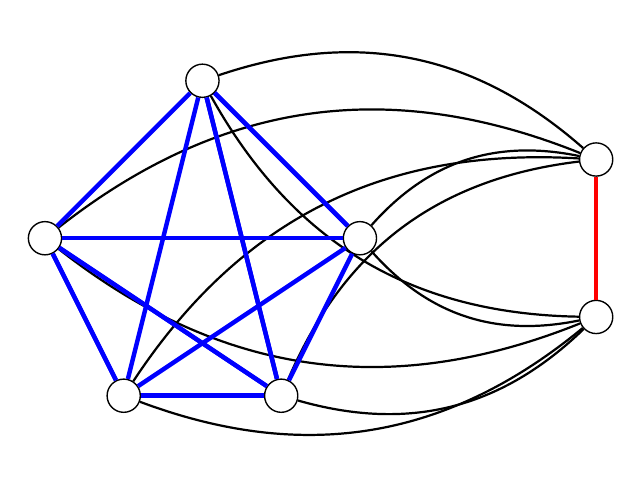
\begin{tikzpicture}
    \SetGraphUnit{2}
    \GraphInit[vstyle=Hasse]
    \Vertex[x=1,y=0]{A}
    \Vertex[x=0,y=2]{B}
    \Vertex[x=2,y=4]{C}
    \Vertex[x=3,y=0]{D}
    \Vertex[x=4,y=2]{E}
    
    \Vertex[x=7, y=3]{F}
    \Vertex[x=7, y=1]{G}
    
    \Edge[style={bend left}](A)(F)
    \Edge[style={bend right}](A)(G)
    
    \Edge[style={bend left}](B)(F)
    \Edge[style={bend right}](B)(G)
    
    \Edge[style={bend left}](C)(F)
    \Edge[style={bend right}](C)(G)
    
    \Edge[style={bend left}](D)(F)
    \Edge[style={bend right}](D)(G)
    
    \Edge[style={bend left}](E)(F)
    \Edge[style={bend right}](E)(G)
    
    \tikzset{EdgeStyle/.style = {ultra thick, color = blue}}
    \Edges(A, B, C, D, E, A, C, D, A, B, D, B, E, C, E)

    \tikzset{EdgeStyle/.style = {ultra thick, color = red}}
    \Edge[](F)(G)
     
\end{tikzpicture}

$G \times H$

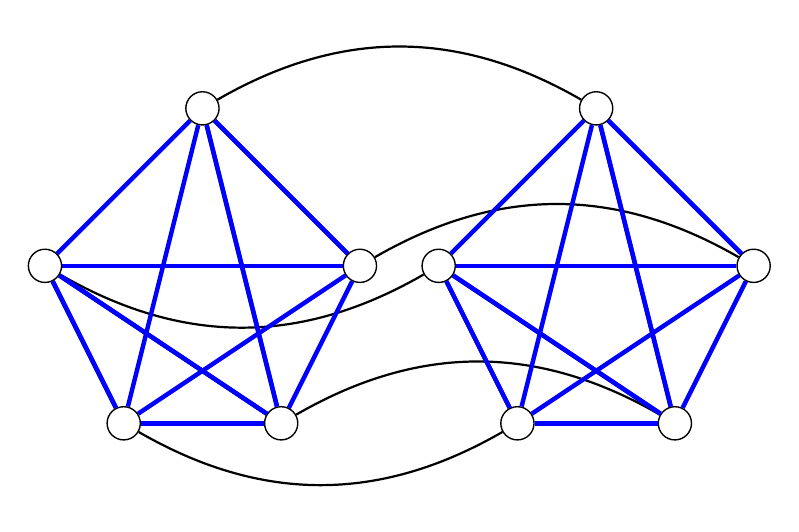
\begin{tikzpicture}
    \SetGraphUnit{2}
    \GraphInit[vstyle=Hasse]
    \Vertex[x=1,y=0]{A}
    \Vertex[x=0,y=2]{B}
    \Vertex[x=2,y=4]{C}
    \Vertex[x=3,y=0]{D}
    \Vertex[x=4,y=2]{E}
    
    \Vertex[x=6,y=0]{1A}
    \Vertex[x=5,y=2]{1B}
    \Vertex[x=7,y=4]{1C}
    \Vertex[x=8,y=0]{1D}
    \Vertex[x=9,y=2]{1E}
    
    \Edge[style={bend right}](A)(1A)
    \Edge[style={bend right}](B)(1B)
    \Edge[style={bend left}](C)(1C)
    \Edge[style={bend left}](D)(1D)
    \Edge[style={bend left}](E)(1E)
   
    \tikzset{EdgeStyle/.style = {ultra thick, color = blue}}
    \Edges(A, B, C, D, E, A, C, D, A, B, D, B, E, C, E)
    \Edges(1A, 1B, 1C, 1D, 1E, 1A, 1C, 1D, 1A, 1B, 1D, 1B, 1E, 1C, 1E) 
\end{tikzpicture}

\subsubsection*{b)}

$\overline{K}_5 + \overline{K}_3$

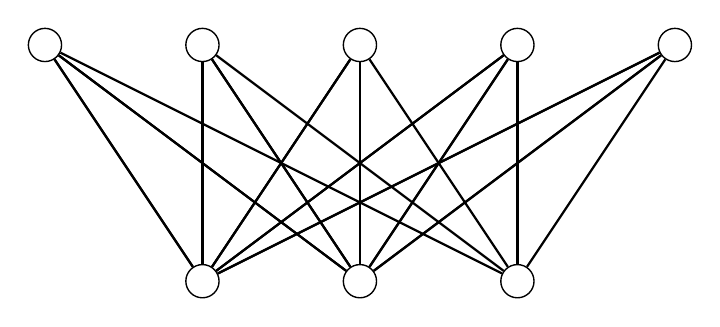
\begin{tikzpicture}

    \SetGraphUnit{2}
    \GraphInit[vstyle=Hasse]
    \Vertex[x=0,y=3]{A}
    \Vertex[x=2,y=3]{B}
    \Vertex[x=4,y=3]{C}
    \Vertex[x=6,y=3]{D}
    \Vertex[x=8,y=3]{E}
    
    \Vertex[x=2,y=0]{F}
    \Vertex[x=4,y=0]{G}
    \Vertex[x=6,y=0]{H}
    
    \Edges(A, F, A, G, A, H)
    \Edges(B, F, B, G, B, H)  
    \Edges(C, F, C, G, C, H)
    \Edges(D, F, D, G, D, H)
    \Edges(E, F, E, G, E, H)

\end{tikzpicture}

$\overline{K}_5 \times \overline{K}_3$

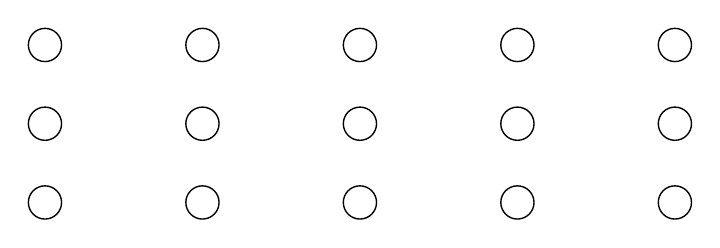
\begin{tikzpicture}
    \SetGraphUnit{2}
    \GraphInit[vstyle=Hasse]
    \Vertex[x=0,y=3]{A}
    \Vertex[x=2,y=3]{B}
    \Vertex[x=4,y=3]{C}
    \Vertex[x=6,y=3]{D}
    \Vertex[x=8,y=3]{E}
    
    \Vertex[x=0,y=2]{1A}
    \Vertex[x=2,y=2]{1B}
    \Vertex[x=4,y=2]{1C}
    \Vertex[x=6,y=2]{1D}
    \Vertex[x=8,y=2]{1E}
    
    \Vertex[x=0,y=1]{2A}
    \Vertex[x=2,y=1]{2B}
    \Vertex[x=4,y=1]{2C}
    \Vertex[x=6,y=1]{2D}
    \Vertex[x=8,y=1]{2E}
\end{tikzpicture}

\subsubsection*{c)}

In the following graphs, the edges of $C_5$ are coloured blue for clarity. \\

$C_5 + K_1$

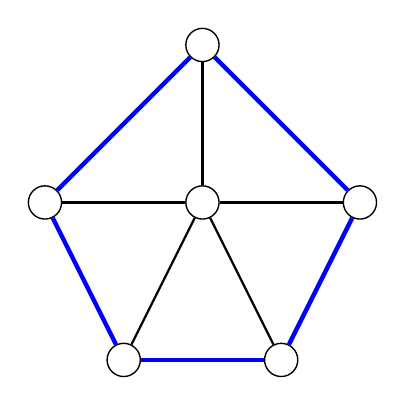
\begin{tikzpicture}
    \SetGraphUnit{2}
    \GraphInit[vstyle=Hasse]
    \Vertex[x=1,y=0]{A}
    \Vertex[x=0,y=2]{B}
    \Vertex[x=2,y=4]{C}
    \Vertex[x=3,y=0]{D}
    \Vertex[x=4,y=2]{E}
    
    \Vertex[x=2,y=2]{F}

    \Edge[](A)(F)
    \Edge[](B)(F)
    \Edge[](C)(F)
    \Edge[](D)(F)
    \Edge[](E)(F)
    
    \tikzset{EdgeStyle/.style = {ultra thick, color = blue}}
    \Edges(A,B,C,E,D,A)
\end{tikzpicture}

$C_5 \times K_1$

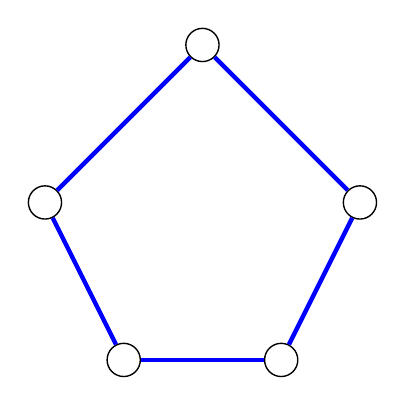
\begin{tikzpicture}
    \SetGraphUnit{2}
    \GraphInit[vstyle=Hasse]
    \Vertex[x=1,y=0]{A}
    \Vertex[x=0,y=2]{B}
    \Vertex[x=2,y=4]{C}
    \Vertex[x=3,y=0]{D}
    \Vertex[x=4,y=2]{E}
    
    \tikzset{EdgeStyle/.style = {ultra thick, color = blue}}
    \Edges(A,B,C,E,D,A)
\end{tikzpicture}

\subsection*{1.16}

\subsection*{1.17}

\subsection*{1.18 b)}

\subsection*{1.19}

\end{document}
